\subsection{Multilevel converter}

\purple{
    Considering a Buck-Boost converter in a Continuous Conduction Mode (CCM) 
    whose topology is shown in Figure \refeq{cap2-circuit-ex-1}. 
}

\begin{figure}[H]
    \centering
    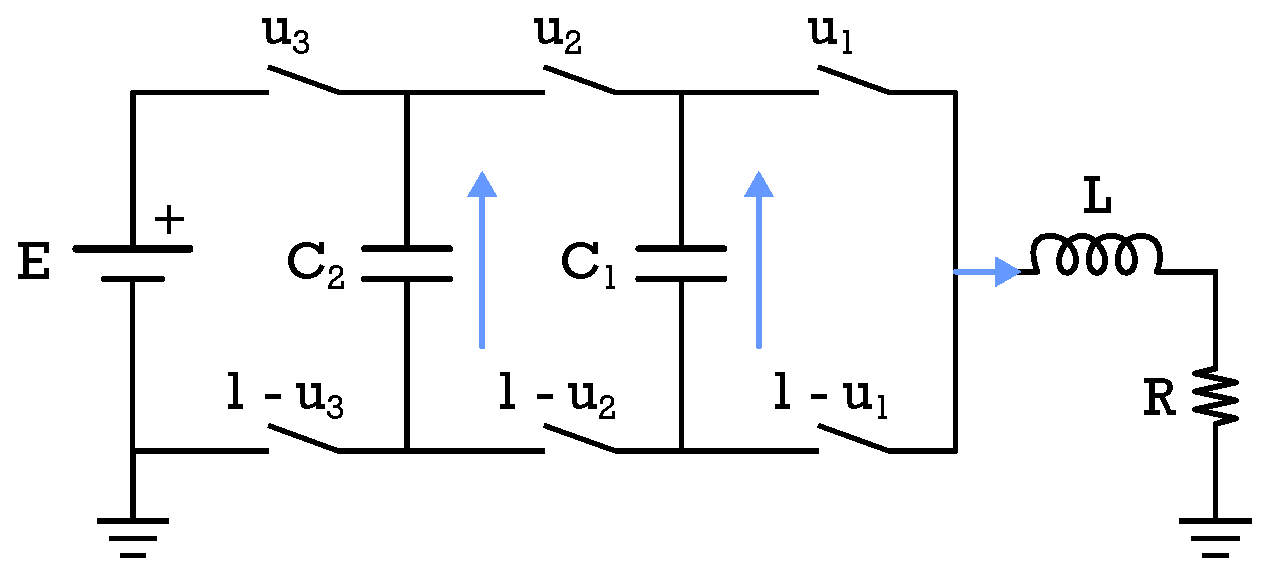
\includegraphics[width=10cm]{Cap2/fig/figura_circuito_ex_2.eps} 
    \caption{Four-level three-cell converter}
    \label{cap2-circuit-ex-2}
\end{figure}

$x(t) = [v_{c_1}(t), v_{c_2}(t), i_L(t)]$. 

\begin{equation}
    \left[ \begin{array}{c}
        \dot{x}_1(t) \\
        \dot{x}_2(t) \\
        \dot{x}_3(t)
    \end{array} \right]
    =
    \left[ \begin{array}{ccc}
        -\frac{x_3(t)}{C_1} & \frac{x_3(t)}{C_1} & 0 \\
        0 & -\frac{x_3(t)}{C_2} & \frac{x_3(t)}{C_2} \\
        \frac{x_1(t)}{L} & \frac{x_2(t) - x_1(t)}{L} & \frac{E - x_2(t)}{L}
    \end{array} \right]
    \left[ \begin{array}{c}
        u_1(t) \\
        u_2(t) \\
        u_3(t)
    \end{array} \right]
    +
    \left[ \begin{array}{c}
        0 \\
        0 \\
        -\frac{R}{L}x_3(t)
    \end{array} \right]
\end{equation}

\begin{equation}
    A = 
    \left[
        \begin{array}{ccc}
            -\frac{x_3(t)}{C_1} & \frac{x_3(t)}{C_1} & 0 \\
            0 & -\frac{x_3(t)}{C_2} & \frac{x_3(t)}{C_2} \\
            \frac{x_1(t)}{L} & \frac{x_2(t) - x_1(t)}{L} & \frac{E-x_2(t)}{L}
        \end{array}
    \right]
\end{equation}

\begin{align}
    \mathbf{u_0} = \left[ \begin{array}{ccc} 0 & 0 & 0 \end{array} \right]^T \\
    \mathbf{u_1} = \left[ \begin{array}{ccc} 0 & 0 & 1 \end{array} \right]^T \\
    \mathbf{u_2} = \left[ \begin{array}{ccc} 0 & 1 & 0 \end{array} \right]^T \\
    \mathbf{u_3} = \left[ \begin{array}{ccc} 0 & 1 & 1 \end{array} \right]^T \\
    \mathbf{u_4} = \left[ \begin{array}{ccc} 1 & 0 & 0 \end{array} \right]^T \\
    \mathbf{u_5} = \left[ \begin{array}{ccc} 1 & 0 & 1 \end{array} \right]^T \\
    \mathbf{u_6} = \left[ \begin{array}{ccc} 1 & 1 & 0 \end{array} \right]^T \\
    \mathbf{u_7} = \left[ \begin{array}{ccc} 1 & 1 & 1 \end{array} \right]^T
\end{align}

\begin{align}
    A_{u_0}=A \mathbf{u_0}&= \left[ \begin{array}{c} 0 \\ 0 \\ \frac{-R x_3(t)}{L} \end{array} \right] = 
    \left[ \begin{array}{ccc} 0&0&0 \\ 0&0&0 \\ 0&0&-\frac{R}{L} \end{array} \right] 
    \left[ \begin{array}{c} x_1(t)\\ x_2(t)\\ x_3(t) \end{array} \right] +
    \left[ \begin{array}{c} 0\\ 0\\ 0 \end{array} \right] \\
    A_{u_1}=A \mathbf{u_1}&= \left[ \begin{array}{c} 0 \\ \frac{x_3(t)}{C_2} \\ \frac{E-x_2(t)-R x_3(t)}{L} \end{array} \right] =
    \left[ \begin{array}{ccc} 0&0&0 \\ 0&0&\frac{1}{C_2} \\ 0&-\frac{1}{L}&-\frac{R}{L} \end{array} \right] 
    \left[ \begin{array}{c} x_1(t)\\ x_2(t)\\ x_3(t) \end{array} \right] +
    \left[ \begin{array}{c} 0\\ 0\\ \frac{E}{L} \end{array} \right] \\
    A_{u_2}=A \mathbf{u_2}&= \left[ \begin{array}{c} \frac{x_3(t)}{C_1} \\ \frac{-x_3(t)}{C_2} \\ \frac{x_2(t)-x_1(t)-R x_3(t)}{L} \end{array} \right] =
    \left[ \begin{array}{ccc} 0&0&\frac{1}{C_1} \\ 0&0&-\frac{1}{C_2} \\ -\frac{1}{L}&\frac{1}{L}&-\frac{R}{L} \end{array} \right]
    \left[ \begin{array}{c} x_1(t)\\ x_2(t)\\ x_3(t) \end{array} \right] +
    \left[ \begin{array}{c} 0\\ 0\\ 0 \end{array} \right] \\
    A_{u_3}=A \mathbf{u_3}&= \left[ \begin{array}{c} \frac{x_3(t)}{C_1} \\ 0 \\ \frac{E-x_1(t)-R x_3(t)}{L} \end{array} \right] =
    \left[ \begin{array}{ccc} 0&0&\frac{1}{C_1} \\ 0&0&\frac{1}{C_2} \\ -\frac{1}{L}&0&-\frac{R}{L} \end{array} \right]
    \left[ \begin{array}{c} x_1(t)\\ x_2(t)\\ x_3(t) \end{array} \right] +
    \left[ \begin{array}{c} 0\\ 0\\ \frac{E}{L} \end{array} \right] \\
    A_{u_4}=A \mathbf{u_4}&= \left[ \begin{array}{c} \frac{-x_3(t)}{C_1} \\ 0 \\ \frac{x_1(t)-R x_3(t)}{L} \end{array} \right] =
    \left[ \begin{array}{ccc} 0&0&\frac{1}{C_1} \\ 0&0&0 \\ -\frac{1}{L}&0&-\frac{R}{L} \end{array} \right]
    \left[ \begin{array}{c} x_1(t)\\ x_2(t)\\ x_3(t) \end{array} \right] +
    \left[ \begin{array}{c} 0\\ 0\\ 0 \end{array} \right] \\
    A_{u_5}=A \mathbf{u_5}&= \left[ \begin{array}{c} \frac{-x_3(t)}{C_1} \\ \frac{x_3(t)}{C_2} \\ \frac{E-x_1(t)-x_2(t)-R x_3(t)}{L} \end{array} \right] =
    \left[ \begin{array}{ccc} 0&0&-\frac{1}{C_1} \\ 0&0&\frac{1}{C_2} \\ \frac{1}{L}&-\frac{1}{L}&-\frac{R}{L} \end{array} \right]
    \left[ \begin{array}{c} x_1(t)\\ x_2(t)\\ x_3(t) \end{array} \right] +
    \left[ \begin{array}{c} 0\\ 0\\ \frac{E}{L} \end{array} \right] \\
    A_{u_6}=A \mathbf{u_6}&= \left[ \begin{array}{c} 0 \\ \frac{-x_3(t)}{C_2} \\ \frac{x_2(t)-R x_3(t)}{L} \end{array} \right] =
    \left[ \begin{array}{ccc} 0&0&0\\ 0&0&-\frac{1}{C_2} \\ 0&\frac{1}{L}&-\frac{R}{L} \end{array} \right]
    \left[ \begin{array}{c} x_1(t)\\ x_2(t)\\ x_3(t) \end{array} \right] +
    \left[ \begin{array}{c} 0\\ 0\\ 0 \end{array} \right] \\
    A_{u_7}=A \mathbf{u_7}&= \left[ \begin{array}{c} 0 \\ 0 \\ \frac{E-R x_3(t)}{L} \end{array} \right] =
    \left[ \begin{array}{ccc} 0&0&0\\ 0&0&0\\ 0&0&-\frac{R}{L} \end{array} \right]
    \left[ \begin{array}{c} x_1(t)\\ x_2(t)\\ x_3(t) \end{array} \right] +
    \left[ \begin{array}{c} 0\\ 0\\ \frac{E}{L} \end{array} \right] \\
\end{align}



% A_u0
\begin{equation}
    \dot{X}=A_{u0}X+b_{0}=
    \left[ \begin{array}{ccc} 0&0&0 \\ 0&0&0 \\ 0&0&-\frac{R}{L} \end{array} \right]
    \left[ \begin{array}{c} x_1(t)\\ x_2(t)\\ x_3(t) \end{array} \right]
    +
    \left[ \begin{array}{c} 0\\ 0\\ 0 \end{array} \right]
\end{equation}

% A_u1
\begin{equation}
    \dot{X}=A_{u1}X+b_{1}=
    \left[ \begin{array}{ccc} 0&0&0 \\ 0&0&\frac{1}{C_2} \\ 0&-\frac{1}{L}&-\frac{R}{L} \end{array} \right]
    \left[ \begin{array}{c} x_1(t)\\ x_2(t)\\ x_3(t) \end{array} \right]
    +
    \left[ \begin{array}{c} 0\\ 0\\ \frac{E}{L} \end{array} \right]
\end{equation}

% A_u2
\begin{equation}
    \dot{X}=A_{u2}X+b_{2}=
    \left[ \begin{array}{ccc} 0&0&\frac{1}{C_1} \\ 0&0&-\frac{1}{C_2} \\ -\frac{1}{L}&\frac{1}{L}&-\frac{R}{L} \end{array} \right]
    \left[ \begin{array}{c} x_1(t)\\ x_2(t)\\ x_3(t) \end{array} \right]
    +
    \left[ \begin{array}{c} 0\\ 0\\ 0 \end{array} \right]
\end{equation}

% A_u3
\begin{equation}
    \dot{X}=A_{u3}X+b_{3}=
    \left[ \begin{array}{ccc} 0&0&\frac{1}{C_1} \\ 0&0&\frac{1}{C_2} \\ -\frac{1}{L}&0&-\frac{R}{L} \end{array} \right]
    \left[ \begin{array}{c} x_1(t)\\ x_2(t)\\ x_3(t) \end{array} \right]
    +
    \left[ \begin{array}{c} 0\\ 0\\ \frac{E}{L} \end{array} \right]
\end{equation}

% A_u4
\begin{equation}
    \dot{X}=A_{u4}X+b_{4}=
    \left[ \begin{array}{ccc} 0&0&\frac{1}{C_1} \\ 0&0&0 \\ -\frac{1}{L}&0&-\frac{R}{L} \end{array} \right]
    \left[ \begin{array}{c} x_1(t)\\ x_2(t)\\ x_3(t) \end{array} \right]
    +
    \left[ \begin{array}{c} 0\\ 0\\ 0 \end{array} \right]
\end{equation}

% A_u5
\begin{equation}
    \dot{X}=A_{u5}X+b_{5}=
    \left[ \begin{array}{ccc} 0&0&-\frac{1}{C_1} \\ 0&0&\frac{1}{C_2} \\ \frac{1}{L}&-\frac{1}{L}&-\frac{R}{L} \end{array} \right]
    \left[ \begin{array}{c} x_1(t)\\ x_2(t)\\ x_3(t) \end{array} \right]
    + \left[ \begin{array}{c} 0\\ 0\\ \frac{E}{L} \end{array} \right]
\end{equation}

% A_u6
\begin{equation}
    \dot{X}=A_{u6}X+b_{6}=
    \left[ \begin{array}{ccc} 0&0&0\\ 0&0&\frac{1}{C_2} \\ 0&-\frac{1}{L}&-\frac{R}{L} \end{array} \right]
    \left[ \begin{array}{c} x_1(t)\\ x_2(t)\\ x_3(t) \end{array} \right]
    +
    \left[ \begin{array}{c} 0\\ 0\\ 0 \end{array} \right]
\end{equation}

% A_u7
\begin{equation}
    \dot{X}=A_{u7}X+b_{7}=
    \left[ \begin{array}{ccc} 0&0&0\\ 0&0&0\\ 0&0&-\frac{R}{L} \end{array} \right]
    \left[ \begin{array}{c} x_1(t)\\ x_2(t)\\ x_3(t) \end{array} \right]
    +
    \left[ \begin{array}{c} 0\\ 0\\ \frac{E}{L} \end{array} \right]
\end{equation}


\purple{
    \noindent
    where
}

\purple{
    \begin{equation}
        \begin{matrix}
            A_1 = \left[ \begin{matrix} 0 & 0 \\ 0 & -\frac{1}{RC} \\ \end{matrix} \right] & 
            A_2 = \left[ \begin{matrix} 0 & \frac{1}{L_1} \\ -\frac{1}{C} & -\frac{1}{RC} \\ \end{matrix} \right] \\
            \\
            b_1 = \left[ \begin{matrix} \frac{E}{L} & 0 \end{matrix} \right]^T & 
            b_2 = \left[ \begin{matrix} 0 & 0 \end{matrix} \right]^T \\
        \end{matrix}
    \end{equation}
}

\purple{
    \noindent
    where $R = L = C = E = 1$. 
}

\purple{
    The list of dynamics for this example is
}

\purple{
    \noindent
    \begin{equation}
        \Big\{\big[A_1,b_1\big], \big[A_2,b_2\big]\Big\}
    \end{equation}
}

\purple{
    \noindent
    where
}

\purple{
    \noindent
    \begin{align}
        A_1 &= \left[
            \begin{matrix}
                0 & 0 \\ 
                0 & 1 \\ 
            \end{matrix}
        \right],
        b_1 = \left[
            \begin{matrix}
                0 \\ 
                1 \\ 
            \end{matrix}
        \right], \\
        A_2 &= \left[
            \begin{matrix}
                0 & 1 \\ 
                -1 & -1 \\ 
            \end{matrix}
        \right],
        b_2 = \left[
            \begin{matrix}
                0 \\ 
                0 \\ 
            \end{matrix}
        \right]
    \end{align}
}

\purple{
    The criteria for the optimization is to compute the trajectory to minimize oscillation around the average value 
    $\big[2,-1\big]$ with the weight matrix $Q = diag\big[1,1\big]$, the maximum cycle period of $T_{p,max} = 1s$ and minimum 
    dwell time of $t_{min} = 0.25s$.

    The cost function takes a vector representing the \( dt \) for each switching moment as its 
    input. For instance, with two switching instances, the vector could be \(\big[ 0.25, 0.35\big]\). 
    This implies the signal begins at time \(0.0\), transitions to the next dynamic at \(0.0 + 0.25 
    = 0.25\), and then switches again at \(0.25 + 0.35 = 0.6\). This gives us the signal sequence 
    \(\big[0.0, 0.25, 0.6\big]\).

    In the Buck-Boost converter example, the initial values for the switching vector are represented 
    by \([0.25, 0.25]\). The lower bounds are defined as \([0.25, 0.25]\) and the upper bounds 
    are set to \([1.5, 1.5]\). The solution provided by the FMINCON optimization yields 
    \(\tau^\infty = \{0, 0.2509, 0.5\}\) and \(\Omega^\infty = \{1, 2\}\).

    The outcome under this condition is displayed in Figure \eqref{cap2-circuit-ex-1}, showcasing 
    the cyclic trajectory around the average value \([2, -1]\). The corresponding command signal 
    can be seen in Figure \eqref{cap2-graf-ex1-2}.
}

\begin{figure}[h!]
    \centering
    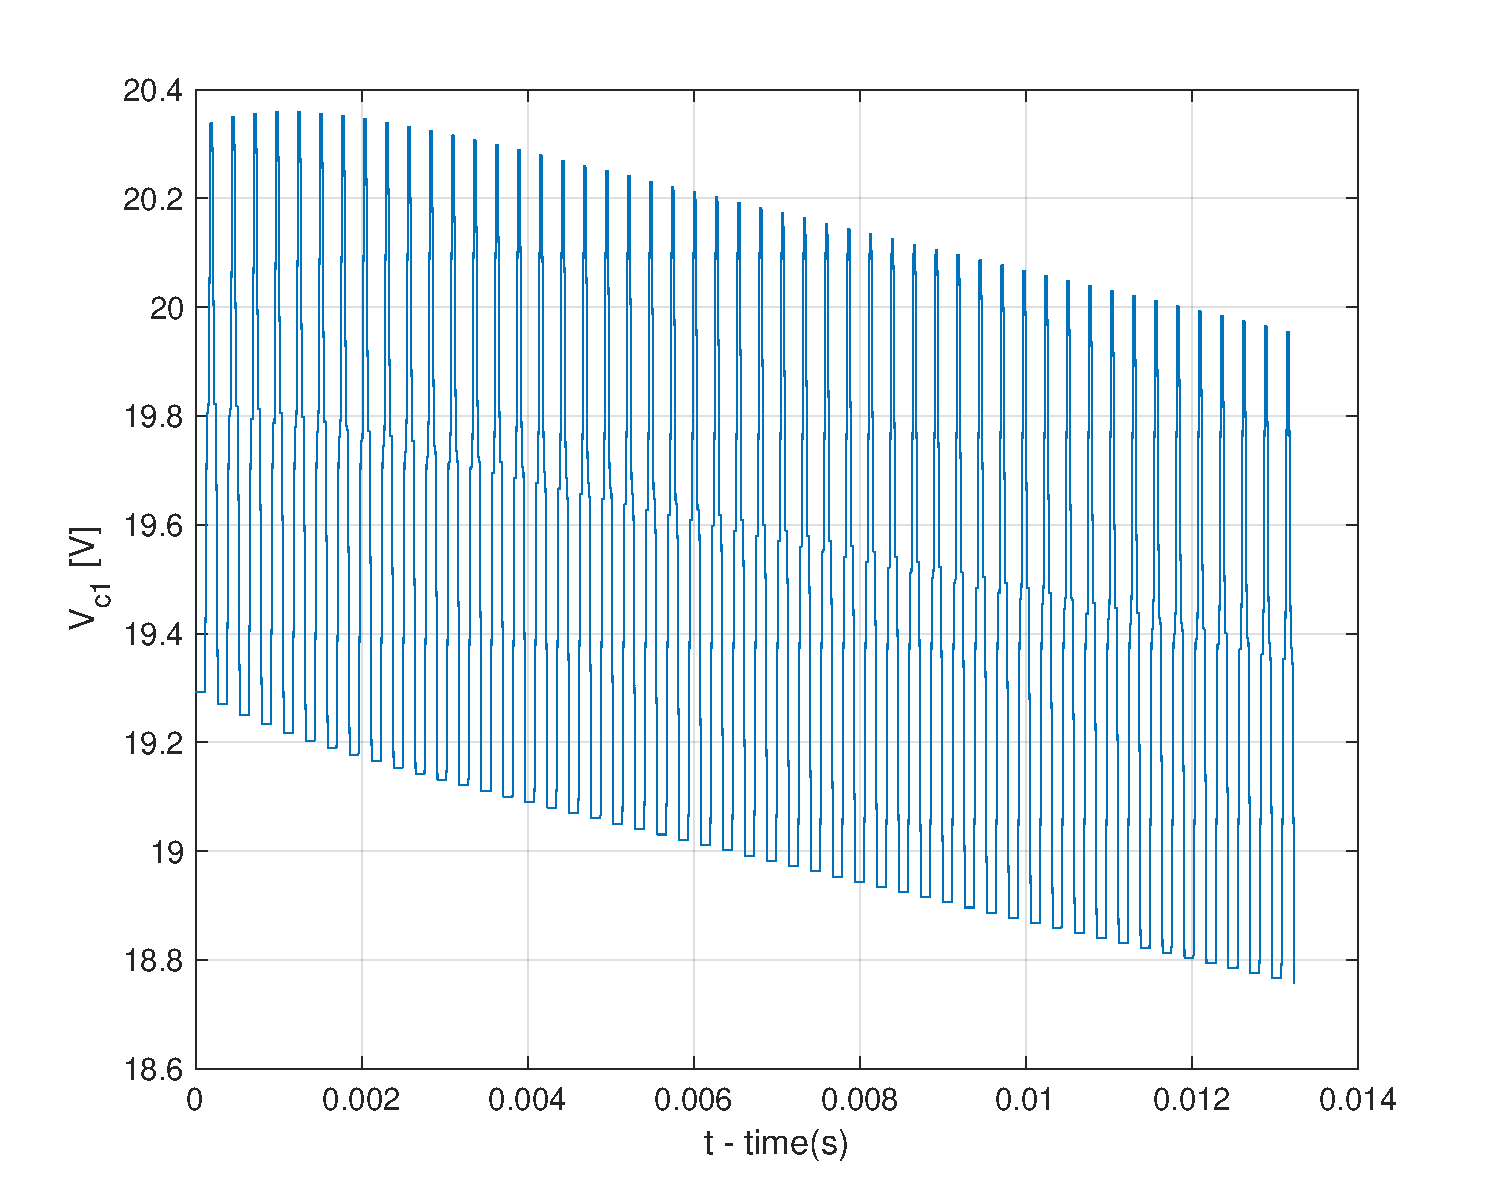
\includegraphics[width=14cm]{Cap2/fig/graf_ex2_1.pdf}
    \caption{Variant Dynamic Circuit 2: Voltage $C_1$}
    \label{cap2-graf-ex2-1}
\end{figure}

\begin{figure}[h!]
    \centering
    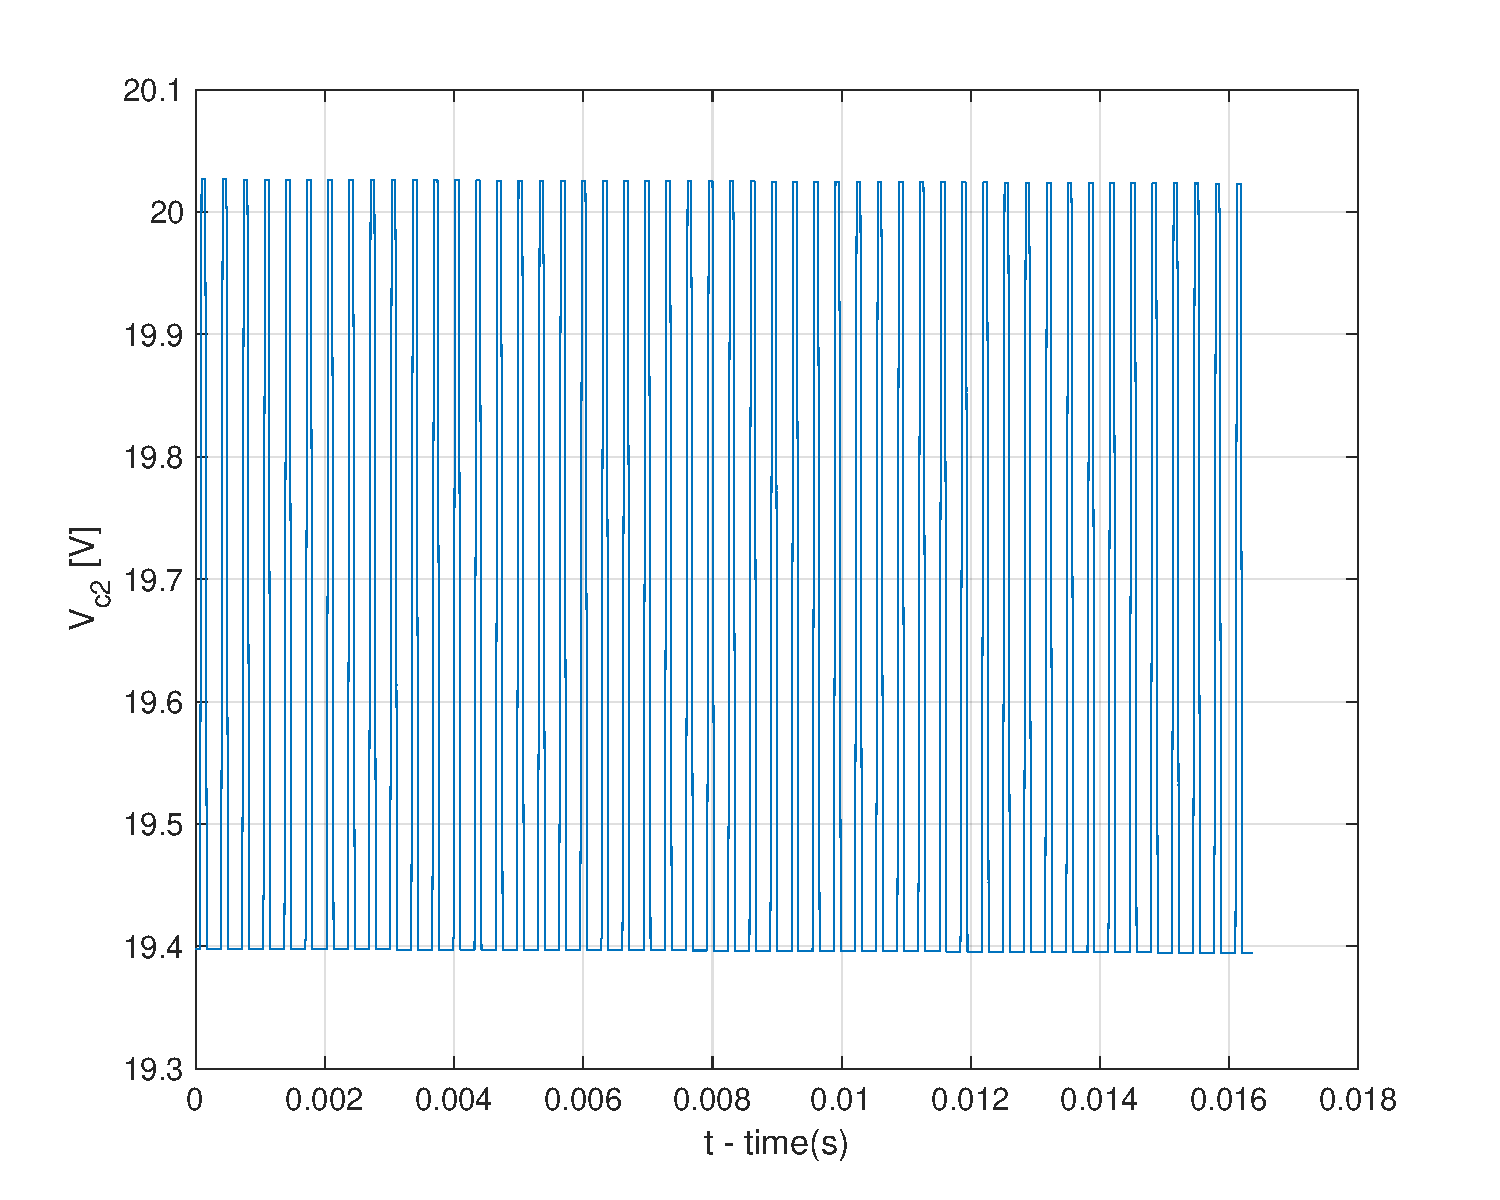
\includegraphics[width=14cm]{Cap2/fig/graf_ex2_2.pdf}
    \caption{Variant Dynamic Circuit 2: Voltage $C_2$}
    \label{cap2-graf-ex2-2}
\end{figure}

\begin{figure}[h!]
    \centering
    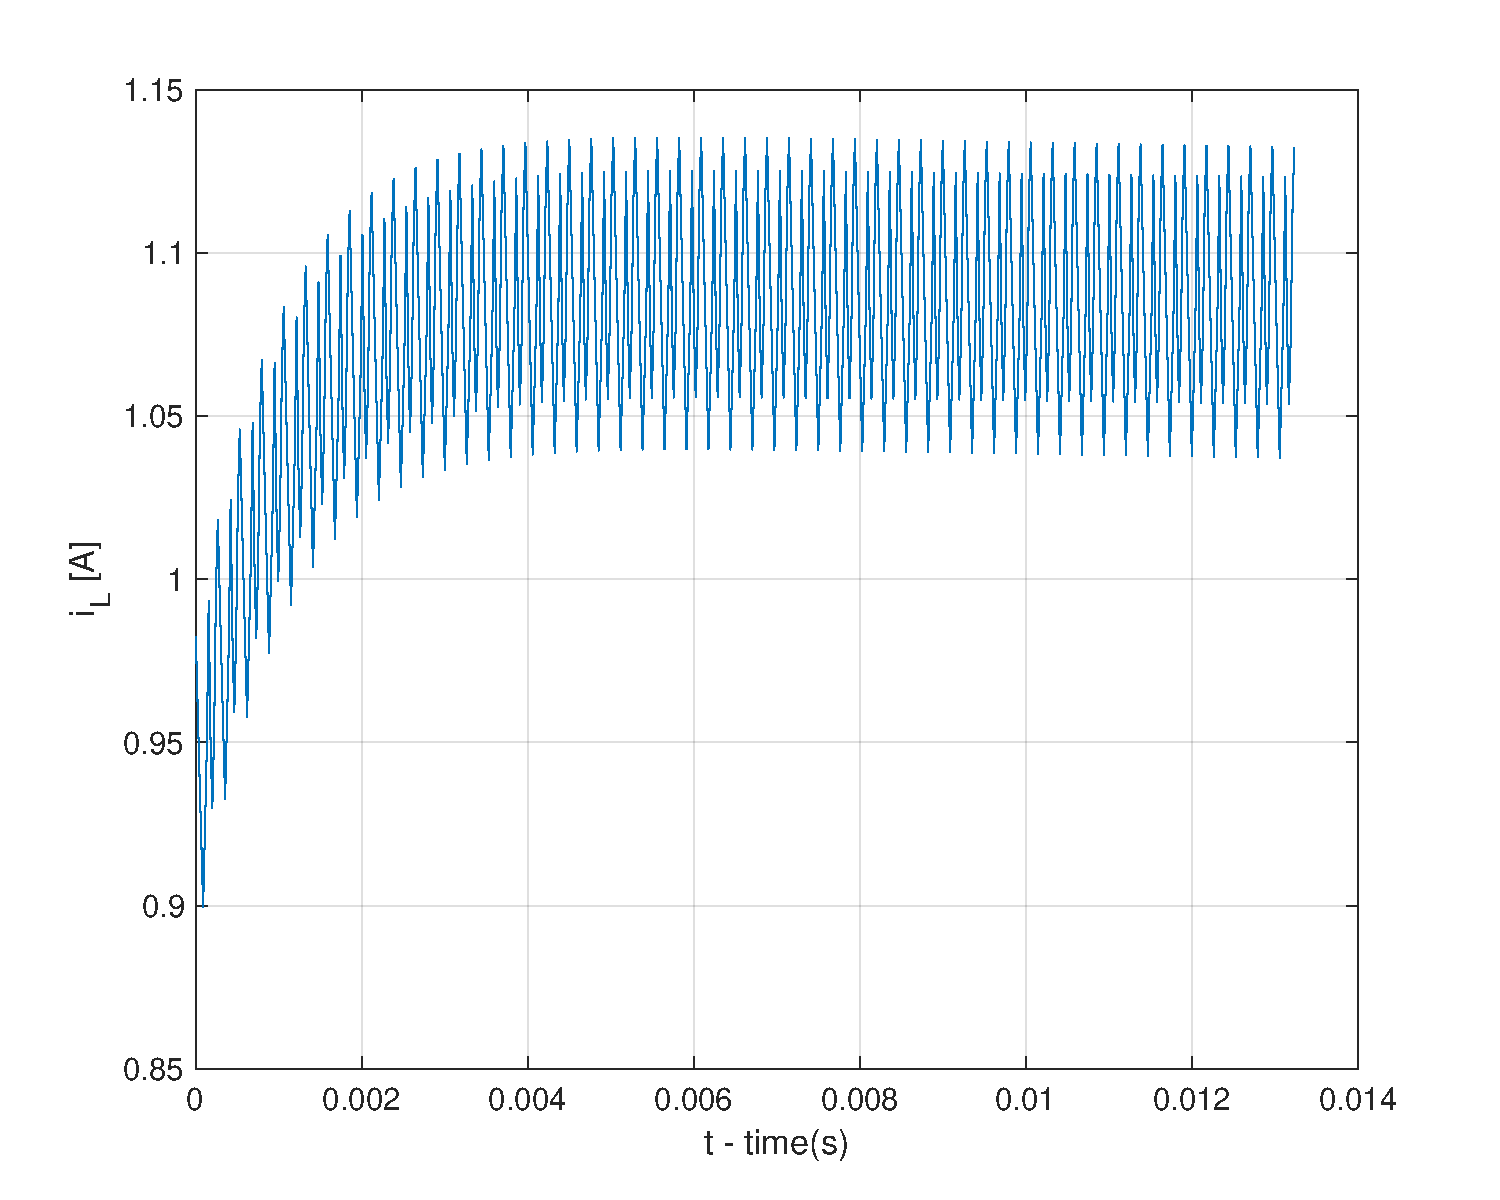
\includegraphics[width=14cm]{Cap2/fig/graf_ex2_3.pdf}
    \caption{Variant Dynamic Circuit 2: Current $L$}
    \label{cap2-graf-ex2-3}
\end{figure}

\begin{figure}[h!]
    \centering
    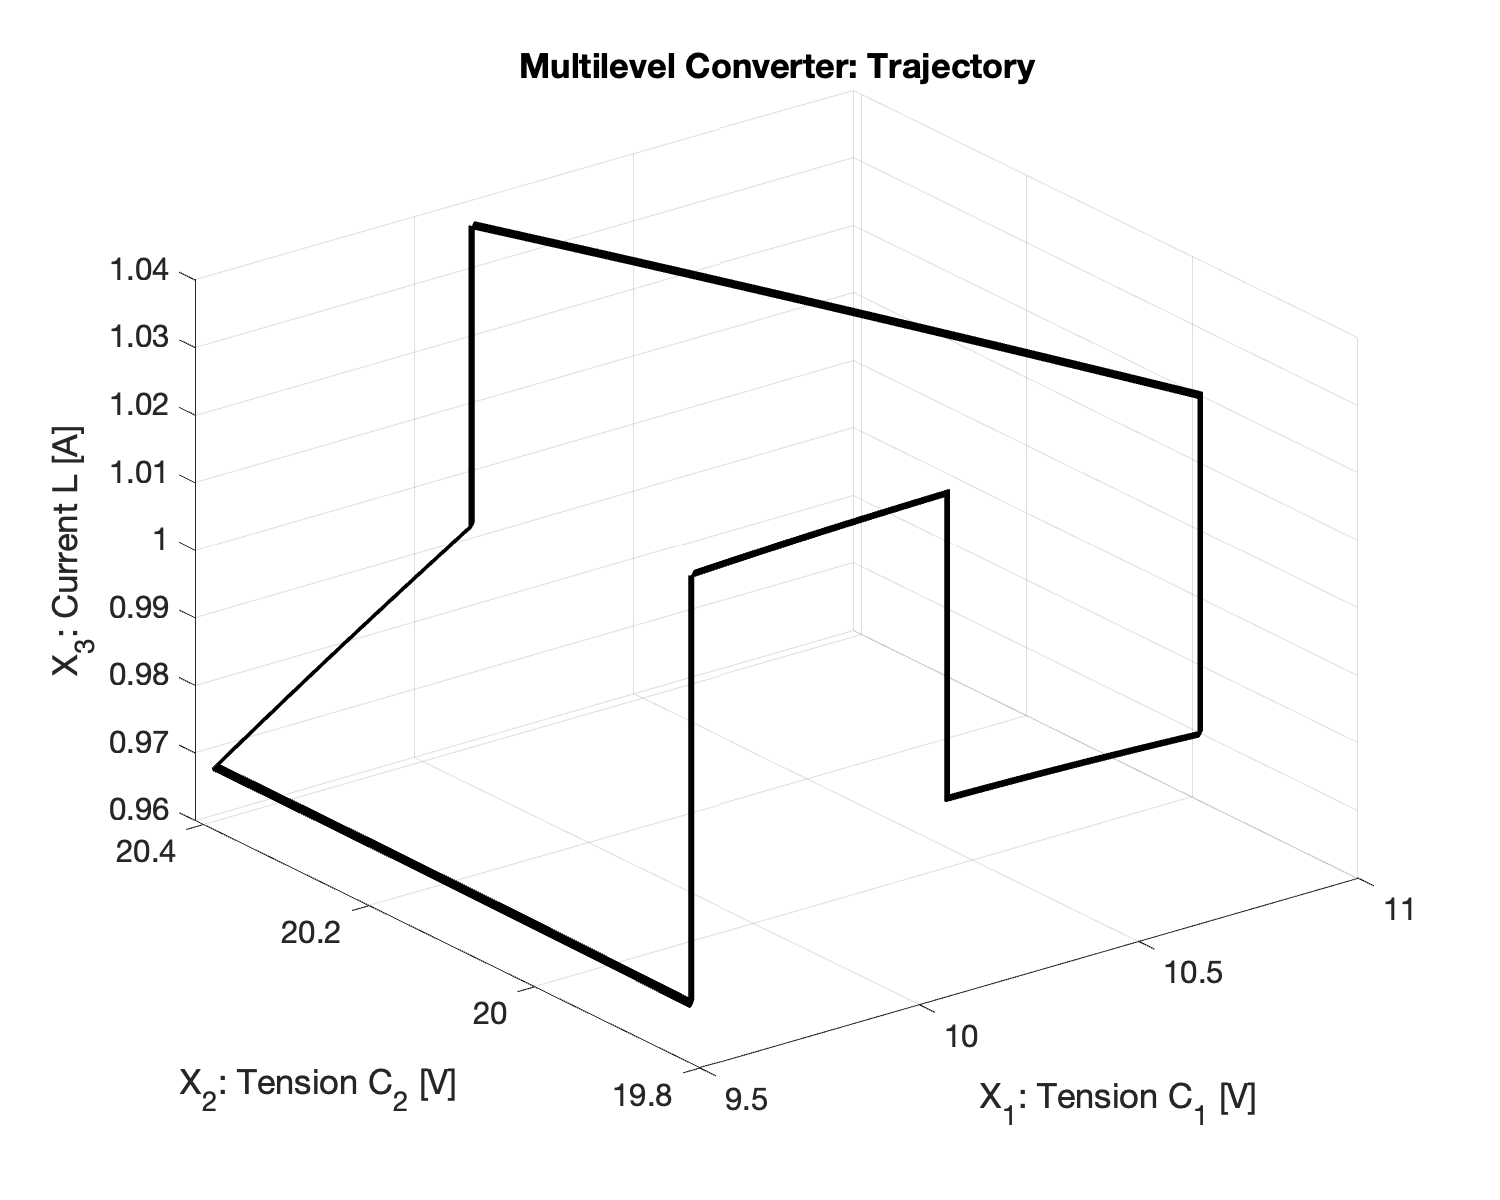
\includegraphics[width=14cm]{Cap2/fig/graf_ex2_4.pdf}
    \caption{Variant Dynamic Circuit 2: State Trajectory}
    \label{cap2-graf-ex2-4}
\end{figure}